\section{Fundamentals of Quantum Computation}%
\label{quantum-computation}

Gate-based quantum computation provides means by which to represent exponentially scaling fermionic wavefunctions using polynomially scaling quantum resources. The fundamental idea that permits this is the ability of quantum devices to encode and manipulate superpositions of states. In contrast, classical computation encodes information using binary strings formed from the computational basis states 0 and 1. For instance, given $n$ classical bits, we can encode $2^n$ binary strings.
\begin{equation*}
    0 \dots 000 = 0 \qquad
    0 \dots 001 = 1 \qquad
    0 \dots 010 = 2 \qquad\dots\qquad
    1 \dots 000 = (2^n - 1)
\end{equation*}

\subsection{Introduction to Qubits}

Information on a quantum computer is encoded using the computational basis states $\ket 0$ and $\ket 1$, known as the $Z$ eigenbasis -- quantum states that correspond to vectors in a two-dimensional complex Hilbert space $\mathbb{C}^2$.
\begin{equation*}
    \ket 0 = \begin{pmatrix} 1 \\ 0 \end{pmatrix} \qquad\qquad
    \ket 1 = \begin{pmatrix} 0 \\ 1 \end{pmatrix} \qquad
\end{equation*}
The state of a given qubit $\ket\psi$ can exist in any superposition of the computational basis states, represented as some complex linear combination of the computational basis states, provided that the qubit state vector is normalised, $\ket\psi = \alpha\ket 0 + \beta\ket 1$ where $|\alpha|^2 + |\beta|^2 = 1$ and $\alpha, \beta \in \mathbb{C}$. A corrollary of this is that we can choose any pair of orthonormal states to form our computational basis. For instance, we define the $X$ eigenbasis as $\ket + = \frac{1}{\sqrt 2} (\ket 0 + \ket 1)$ and $\ket - = \frac{1}{\sqrt 2} (\ket 0 - \ket 1)$.

\begin{figure}[H]
    \centering
    \begin{minipage}{.23\textwidth}
        \centering
        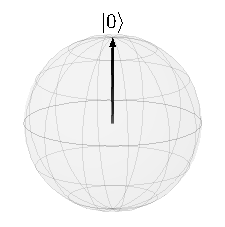
\includegraphics[width=0.7\linewidth]{chapter-1/zero}
    \end{minipage}%
    \begin{minipage}{0.23\textwidth}
        \centering
        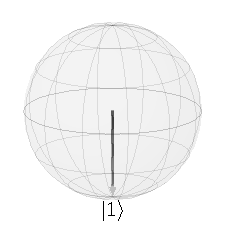
\includegraphics[width=0.7\linewidth]{chapter-1/one}
    \end{minipage}
    \begin{minipage}{0.23\textwidth}
        \centering
        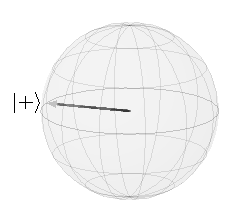
\includegraphics[width=0.8\linewidth]{chapter-1/plus}
    \end{minipage}
    \begin{minipage}{0.23\textwidth}
        \centering
        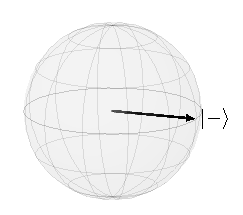
\includegraphics[width=0.8\linewidth]{chapter-1/minus}
    \end{minipage}
    \caption{Bloch sphere representations of the $Z$ (left) and $X$ (right) eigenbases.}
\end{figure}

Whilst a single qubit can exist in an infinite number of states, upon measuring the qubit state with respect to a particular basis, the qubit state collapses into one computational basis state or the other. This gives rise to the \textit{no-cloning theorem}, which states that it is impossible to create an indentical and independent copy of an arbitrary unknown quantum state, as this would involve first measuring that state.

Let us now consider systems consisting of multiple qubits. Similarly to how $n$ classical bits give rise to $2^n$ binary strings, we have that $n$ qubits give rise to $2^n$ basis states. These basis states are formed by taking the Kronecker. For instance, a two-qubit system gives rise to the four following basis states.
\begin{equation*}
    \ket{00} = \ket 0 \otimes \ket 0 \qquad
    \ket{01} = \ket 0 \otimes \ket 1 \qquad
    \ket{10} = \ket 1 \otimes \ket 0 \qquad
    \ket{11} = \ket 1 \otimes \ket 1
\end{equation*}
An arbitrary $n$-qubit \textit{state vector} describing the state of the entire system can be formed by taking a complex linear combination of the $2^n$ basis states. Therefore, in order to fully describe an arbitrary $n$-qubit state vector, we need to specify $2^n$ complex coefficients. In the case of a two-qubit system, we have the following.
\begin{gather*}
    \ket\psi =
    \alpha \ket{00} +
    \beta \ket{01} +
    \gamma \ket{10} +
    \delta \ket{11} \\
    \text{where} \,\,\,\, \alpha, \, \beta, \, \gamma, \, \delta \in \mathbb{C}
\end{gather*}

\subsection{Introduction to Quantum Gates}%
\label{quantum-gates}

Quantum gates, by definition, correspond to unitary transformations, $U^{-1} = U^\dagger$ \cite{Nielsen2012}. In other words, any quantum gate corresponds to a square unitary matrix that conserves the complex inner product of the state it acts on. Consequently, quantum gates can be viewed as rotations of the qubit state vector in Hilbert space.

We will now introduce the Pauli matrices, which are the most fundamental gates in quantum computing. They are implemented on a quantum device as the Pauli gates, and correspond to $2 \times 2$ matrices that rotate their input by $\pi$ radians in their respective basis. We define the Pauli matrices as follows.

\begin{figure}[H]
    \centering
    \begin{equation*}
        I = \begin{pmatrix} 1 & 0 \\ 0 & 1\end{pmatrix} \qquad
        X = \begin{pmatrix} 0 & 1 \\ 1 & 0\end{pmatrix} \qquad
        Y = \begin{pmatrix} 0 & -i \\ i & \,\,\,\,0\end{pmatrix} \qquad
        Z = \begin{pmatrix} 1 & \,\,\,0 \\ 0 & -1\end{pmatrix}
    \end{equation*}
    \caption{The Pauli matrices.}
    \label{pauli-matrices}
\end{figure}

The Pauli $X$ gate is the quantum analogue of the classical NOT gate in that it maps $\ket 0$ to $\ket 1$ and $\ket 1$ to $\ket 0$. Importantly, the Pauli gates differ from their classical counterparts in that they can act on any arbitrary qubit state $\ket\psi$. Similarly, the Pauli $Z$ gate maps $\ket +$ to $\ket -$ and \textit{vice versa}.

\begin{figure}[H]
    \centering
    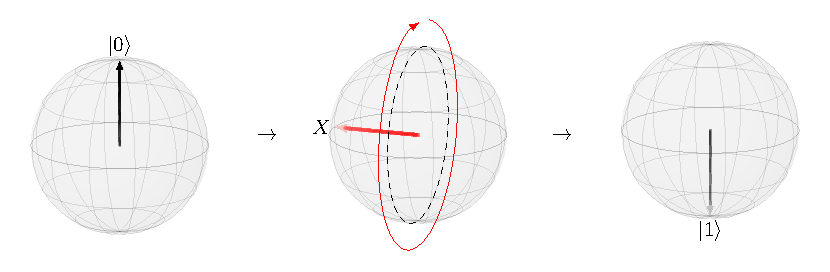
\includegraphics[width=0.6\linewidth]{chapter-1/zero_one}
    \caption{Pauli $X$ gate acting on the $\ket 0$ state.}
\end{figure}

An important gate that we will make extensive use of is the Hadamard gate, which maps $\ket 0$ to $\ket +$ and \textit{vice versa}, as well as $\ket 1$ to $\ket -$ and \textit{vice versa}. The Hadamard gate, interconverts between the $Z$ and $X$ bases through a rotation $\pi$ radians about the line bisecting the $z$ and $x$ axes in the Bloch sphere representation.

\begin{figure}[H]
    \centering
    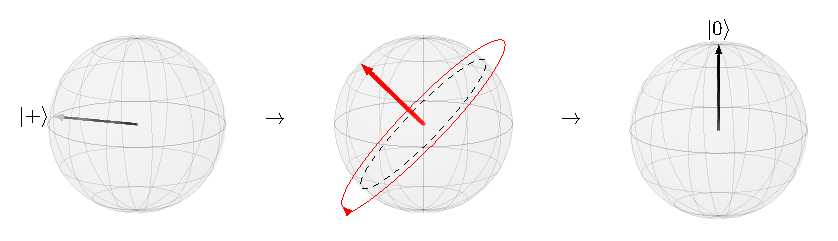
\includegraphics[width=0.6\linewidth]{chapter-1/plus_zero}
    \caption{Hadamard gate acting on the $\ket +$ state.}
\end{figure}

Recall that all quantum gates are untitary, by definition, and since the quantum gates that we have discussed so far are Hermitian, $H = H^\dagger$, it follows that they are also self-inverse. Therefore, sequentially applying any of the quantum gates discussed so far is equivalent to applying no transformation.

The R$_Z(\theta)$ and R$_X(\theta)$ rotation gates correspond to rotations of the Bloch sphere by some arbitrary angle $\theta$, in the $Z$ and $X$ bases respectively.

\begin{figure}[H]
    \centering
    \begin{minipage}{0.45\textwidth}
        \centering
        \includezxdiagramtext{chapter-1/z_rotation}{0.4}{
        \begin{pmatrix} 1 & 0 \\ 0 & e^{i\theta} \\ \end{pmatrix}}
    \end{minipage}
    \begin{minipage}{0.45\textwidth}
        \centering
        \includezxdiagramtext{chapter-1/x_rotation}{0.35}{
        \begin{pmatrix}
              1 + e^{i\theta} & 1 - e^{i\theta} \\
              1 - e^{i\theta} & 1 + e^{i\theta}
        \end{pmatrix}}
    \end{minipage}
    \caption{Arbitrary rotations in the $Z$ and $X$ bases by $\theta$ radians.}
\end{figure}

We will now introduce the two-qubit CNOT gate, which is used to entangle two qubits. Consider a two-qubit state of the form $\ket \alpha \otimes \ket \beta$. We define CNOT as the gate that takes $\alpha$ to be the control qubit and $\beta$ to be the target qubit, and acts on the $\ket\alpha\otimes\ket\beta$ state to give the $\ket\alpha\otimes\ket{\alpha\oplus\beta}$ state. That is, the CNOT gate applies the Pauli $X$ gate to the target qubit \textit{iff} the control qubit is in the $\ket 1$ state. The CNOT gate acts on the two-qubit basis states as follows.
\begin{equation*}
    \ket{00} \rightarrow \ket {00} \qquad
    \ket{01} \rightarrow \ket {01} \qquad
    \ket{10} \rightarrow \ket {11} \qquad
    \ket{11} \rightarrow \ket {10}
\end{equation*}
In this way the CNOT gate is the quantum generalisation of the classical XOR gate. Since the CNOT must be unitary, it has two outputs instead of one, such that $\text{CNOT}^{-1}$ is well-defined. We define the matrices corresponding to the CNOT gates, with the control and target qubits interchanged, as follows.
\begin{equation*}
\text{CNOT}^{c=0}_{t=1} =
    \begin{pmatrix}
        1 & 0 & 0 & 0 \\
        0 & 1 & 0 & 0 \\
        0 & 0 & 0 & 1 \\
        0 & 0 & 1 & 0
    \end{pmatrix} \qquad
    %
    \text{CNOT}^{c=1}_{t=0} =
    \begin{pmatrix}
        1 & 0 & 0 & 0 \\
        0 & 0 & 0 & 1 \\
        0 & 0 & 1 & 0 \\
        0 & 1 & 0 & 0
    \end{pmatrix}
\end{equation*}\smallskip
The CNOT gate can be used to entangle two qubits when the control qubit exists in a superposition of states. For instance, the CNOT gate actions on the $\ket{+0}$ state to give the $\frac{1}{\sqrt 2} (\ket{00} + \ket{11})$ Bell state.
